\section{Лекция 2}

В зависимости от знака перед $i\varepsilon$, введем:
\[
G_0^{(\pm)}\!\Bigl(E = \tfrac{\vec{p}^2}{2m},\,\vec{r},\,\vec{r'}\Bigr)
= \dfrac{m}{2i\pi^2\hbar^2}\cdot\dfrac{1}{|\vec{r}-\vec{r'}|}
\int_{-\infty}^{\infty} dp'\,\dfrac{p'\,e^{\frac{i}{\hbar}\,p'|\vec{r}-\vec{r'}|}}{p^2 - (p')^2 \pm i\widetilde{\varepsilon}},
\quad \widetilde\varepsilon > 0
\]

Рассмотрим
\[
G_0^{(+)}\!\Bigl(E = \tfrac{\vec{p}^2}{2m},\,\vec{r},\,\vec{r'}\Bigr)
= \dfrac{m}{2i\pi^2\hbar^2}\cdot\dfrac{1}{|\vec{r}-\vec{r'}|}
\int_{-\infty}^{\infty} dp'\,\dfrac{p'\,e^{\frac{i}{\hbar}\,p'|\vec{r}-\vec{r'}|}}{p^2 - (p')^2 + i\widetilde{\varepsilon}} = (*)
\]

Заметим, что при $\widetilde{\varepsilon} << 1$ знаменатель принимает вид
\[
p^2 - (p')^2 + i\widetilde{\varepsilon} \approx (p + i\widetilde{\widetilde{\varepsilon}} - p')(p + i\widetilde{\widetilde{\varepsilon}} + p'), \quad \widetilde{\widetilde{\varepsilon}} > 0, \, \widetilde{\widetilde{\varepsilon}}<<1
\]

$\Rightarrow$ 2 полюса: $p' = p + i\widetilde{\widetilde{\varepsilon}}$ и $p' = -p - i\widetilde{\widetilde{\varepsilon}}$.

\begin{figure}[H]
	\centering
	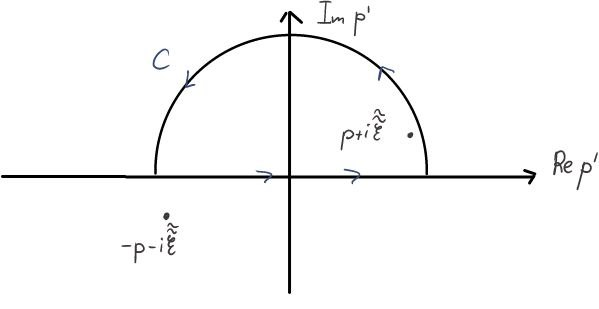
\includegraphics[width=0.75\linewidth]{images/l2_1.jpg}
\end{figure}

\[
(*) = -\dfrac{m}{2i\pi^2\hbar^2}\cdot\frac{1}{|\vec{r}-\vec{r'}|}
\oint_C dp'\,\frac{p'\,e^{\frac{i}{\hbar}\,p'|\vec{r}-\vec{r}'|}}{(p' - p - i\widetilde{\widetilde{\varepsilon}})(p' + p + i\widetilde{\widetilde{\varepsilon}})}
\implies \text{итого}
\]

\[
G_0^{(+)}\!\Bigl(E = \tfrac{\vec{p}^2}{2m},\,\vec{r},\,\vec{r'}\Bigr)
= -\frac{m}{2\pi\hbar^2}\,\frac{pe^{+\frac{i}{\hbar}\,p|\vec{r}-\vec{r'}|}}{|\vec{r}-\vec{r'}|}
\]

Аналогично:
\[
G_0^{(-)}\!\Bigl(E = \tfrac{\vec{p}^2}{2m},\,\vec{r},\,\vec{r'}\Bigr)
= -\frac{m}{2\pi\hbar^2}\,\frac{pe^{-\frac{i}{\hbar}\,p|\vec{r}-\vec{r'}|}}{|\vec{r}-\vec{r'}|}
\]


\subsection{\S XII.4. Связь операторов $\hat{H}$ и $\hat{H}_0$}

Пусть $\hat{H}_0$ --- это невозмущённый гамильтониан.

\begin{proposition}
	$\hat{A}^{-1} = \hat{B}^{-1}(\hat{1} + (\hat{B} - \hat{A})\,\hat{A}^{-1})$
\end{proposition}

\begin{proof}
	\[
	\hat{A}^{-1} - \hat{B}^{-1}
	= \hat{1}\hat{A}^{-1} - \hat{B}^{-1}\hat{1} = \hat{B}^{-1}\hat{B}\hat{A}^{-1}
	- \hat{B}^{-1}\hat{A}\hat{A}^{-1}
	= \hat{B}^{-1}(\hat{B} - \hat{A})\hat{A}^{-1}
	\]
\end{proof}

Пусть $\hat{A} = \hat{G}^{-1}(z) = \hat{1}z - \hat{H}$,\quad
$\hat{B} = \hat{G}_0^{-1}(z) = \hat{1}z - \hat{H}_0$\quad
$\Rightarrow\; \hat{B} - \hat{A} = \hat{H} - \hat{H}_0 = \hat{V}$ $\Rightarrow$ по утверждению выше верно, что

\[
\hat{G}(z) = \hat{G}_0(z)\!\left(\hat{1} + \hat{V}(t)\right)\hat{G}(z)
\]

Будем решать методом итераций:
\begin{align*}
	\hat{G}^{(1)}(z) &= \hat{G}_0 + \hat{G}_0\,\hat{V}\,\hat{G}_0\\
	\hat{G}^{(2)}(z) &= \hat{G}_0 + \hat{G}_0\,\hat{V}\,\hat{G}_0 + \hat{G}_0\,\hat{V}\,\hat{G}_0\,\hat{V}\,\hat{G}_0\\
	&\;\vdots
\end{align*}

$\Rightarrow \hat{G}(z)$ может быть записана $2^{\text{мя}}$ способами:
\begin{enumerate}
	\item $\hat{G}(z) = \hat{G}_0(z)\Bigl(\hat{1} + \displaystyle\sum_{s=1}^\infty\bigl(\hat{V}(t)\hat{G}_0(z)\bigr)^s\Bigr)$
	\item $\hat{G}(z) = \Bigl(\hat{1} + \displaystyle\sum_{s=1}^\infty\bigl(\hat{G}_0(z)\,\hat{V}(t)\bigr)^s\Bigr)\hat{G}_0(z)$
\end{enumerate}

\subsection{\S XII.5. Стационарная теория возмущений для невырожденного спектра}

В этом параграфе сделаем следующие предположения:

\begin{enumerate}[label=\alph*)]
	\item Пусть гамильтониан полной системы $\hat{H}$, гамильтониан невозмущенной системы $\hat{H}_0$ и  возмущение $\hat{V}$ от времени $t$ не зависят.
	\item Пусть $\hat{H}$ и $\hat{H}_0$ имеют дискретный неырожденный спектр.
\end{enumerate}

\begin{figure}[H]
	\centering
	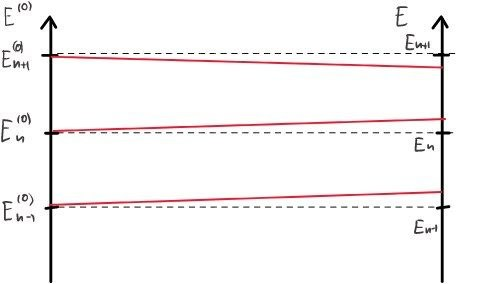
\includegraphics[width=0.75\linewidth]{images/l2_2.jpg}
\end{figure}

Рассмотрим уровни энергии $\hat{H}\ket{E_n} = E_n\ket{E_n}$, \quad $\hat{H}_0\ket{E_n^{(0)}} = E_n^{(0)}\ket{E_n^{(0)}}$. Мы хотим построить стационарную теорию возмущений, для этого нам надо, чтобы уровни сдвигались "немного". Это "немного" определим, добавив третье предположение:
\begin{enumerate}[label=\alph*)]
	\item[c)]  $\bigl|E_n - E_n^{(0)}\bigr| \ll \tfrac{1}{2}\bigl\{|E_n - E_{n-1}|,\; |E_{n+1} - E_n|,\; |E_n^{(0)} - E_{n-1}^{(0)}|,\; |E_{n+1}^{(0)} - E_{n}^{(0)}|\bigr\}$.
\end{enumerate}

Тогда $\forall n \hookrightarrow E_n = E_n^{(0)} + \delta E_n = E_n^{(0)} + \delta E_n^{(1)} + \delta E_n^{(2)} + \ldots$\\




Поскольку спектры $\hat{H}$ и $\hat{H}_0$ дискретны и невырождены, то:
\[
\hat{G}_0(z) = \sum_n \frac{\ket{E_n^{(0)}}\bra{E_n^{(0)}}}{z - E_n^{(0)}} = \sum_n \frac{\hat{P}_{E_n^{(0)}}}{z - E_n^{(0)}}
\]
\[
\hat{G}_0(z)\ket{E_k^{(0)}} = \sum_n \frac{\ket{E_n^{(0)}}\braket{E_n^{(0)}}{E_k^{(0)}}}{z - E_n^{(0)}} = \frac{\ket{E_k^{(0)}}}{z - E_k^{(0)}}
\]

Для полного гамильтониана:
\[
\hat{G}(z) = \sum_n \frac{\hat{P}_{E_n}}{z - E_n}
= \left(\hat{1} + \sum_s \bigl(G_0(z)\,\hat{V}\bigr)^s\right)\hat{G}_0(z), \quad \hat{V} \neq \hat{V}(t)
\]


Рассмотрим оператор $\hat{A}(z)$ без особенностей (в частности, без полюсов).
\begin{figure}[H]
	\centering
	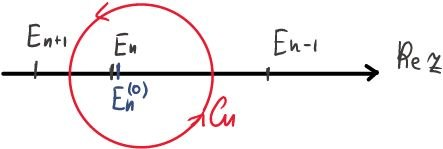
\includegraphics[width=0.75\linewidth]{images/l2_3.jpg}
\end{figure}
Тогда 
\[
\oint_{C_n} dz\,\hat{A}(z)\,\hat{G}(z)
= \oint_{C_n} dz\,\frac{\hat{A}(z)\,\hat{P}_{E_n}}{z - E_n}
= 2\pi i\,\hat{A}(E_n)\,\hat{P}_{E_n}
\]

Посчитаем поправку к уровням энергии.

\begin{align*}
	\bigl(E_n^{(0)} + \delta E_n\bigr)\bra{E_n^{(0)}}\hat{P}_{E_n}\ket{E_n^{(0)}} = \\
	&= E_n \bra{E_n^{(0)}}\hat{P}_{E_n}\ket{E_n^{(0)}} = \\
	&= \bra{E_n^{(0)}} E_n \hat{P}_{E_n}\ket{E_n^{(0)}}
	= \bra{E_n^{(0)}} \hat{H}\hat{P}_{E_n}\ket{E_n^{(0)}} = \\
	&= \bra{E_n^{(0)}} (\hat{H}_0 + \hat{V})\hat{P}_{E_n}\ket{E_n^{(0)}} = \\
	&= E_n^{(0)}\bra{E_n^{(0)}}\hat{P}_{E_n}\ket{E_n^{(0)}} + \bra{E_n^{(0)}}\hat{V}\hat{P}_{E_n}\ket{E_n^{(0)}}
\end{align*}

Итого 
\[
\boxed{
	\delta E_n = \dfrac{\bra{E_n^{(0)}}\hat{V}\hat{P}_{E_n}\ket{E_n^{(0)}}}{\bra{E_n^{(0)}}\hat{P}_{E_n}\ket{E_n^{(0)}}}
}
\]

--- точная формула поправки к $E_n$. Хотим найти поправки вплоть до $2^\text{го}$ порядка.\\

Вычислим числитель $\bra{E_n^{(0)}}\hat{V}\hat{P}_{E_n}\ket{E_n^{(0)}}$:
\[
\bra{E_n^{(0)}}\hat{V}\hat{P}_{E_n}\ket{E_n^{(0)}} = \frac{1}{2\pi i}\bra{E_n^{(0)}}\oint_{C_n} dz\,\hat{V}\hat{G}(z)\ket{E_n^{(0)}}
	= \frac{1}{2\pi i}\oint_{C_n} dz\,\bra{E_n^{(0)}}\hat{V}\hat{G}_0(z) + \hat{V}\hat{G}_0\hat{V}\hat{G}_0 + \ldots\ket{E_n^{(0)}} = 
\]
\[
= \frac{1}{2\pi i}\Big(\oint_{C_n} dz\dfrac{\braupket{E_n^{(0)}}{\hat{V}{E_n^{(0)}}}{z-E_n^{(0)}}} + \oint_{C_n}dz \braupket{E_n^{(0)}}{\hat{V}\hat{G}_0\hat{1}\hat{V}\hat{G}_0}{E)n^{(0)}} + \ldots\Big) = (*) 
\]

Пусть $\hat{V}_{mn} = \braupket{E_m^{(0)}}{\hat{V}}{E_n^{(0)}}$

\[
(*) = \frac{1}{2\pi i} \Big(\oint_{C_n} dz \dfrac{V_{nn}}{z - E_n^{(0)}} + \oint_{C_n} dz \sum\limits_{m\neq n}\dfrac{V_{nm}V_{mn}}{(z - E_m^{(0)})(z - E_n^{(0)})} + \oint_{C_n} dz \dfrac{|V_{nn|^2}}{(z - E_n^{(0)})^2}\Big) = 
\]
\[
= V_{nn} + \sum\limits_{m\neq n}\dfrac{V_{nm}V_{mn}}{E_n^{(0)} - E_m^{(0)}} + \underbrace{2\pi i \lim\limits_{z \longrightarrow E_n^{(0)}} \frac{d}{dz} |V_{nn}|^2}_{\text{= 0}} + \ldots
\]


$\Rightarrow \bra{E_n^{(0)}}\hat{V}\hat{P}_{E_n}\ket{E_n^{(0)}} = V_{nn} + \sum\limits_{m \neq n} \dfrac{|V_{nm}|^2}{E_n^{(0)} - E_m^{(0)}}$.

Знаменатель $\bra{E_n^{(0)}}\hat{P}_{E_n}\ket{E_n^{(0)}} = 1 + \ldots$ $\Rightarrow$

\[
\delta E_n = \delta E_n^{(1)} + \delta E_n^{(2)} + \ldots = V_{nn} + \sum_{m \neq n} \frac{|V_{nm}|^2}{E_n^{(0)} - E_m^{(0)}}
\]

\[
\Rightarrow E_n = E_n^{(0)} + V_{nn} + \sum_{m \neq n} \frac{|V_{nm}|^2}{E_n^{(0)} - E_m^{(0)}}
\]

Если у $\hat{H}_0$ добавляется непрерывный спектр, то 
\[
E_n = E_n^{(0)} + V_{nn} + \displaystyle\sum_{m \neq n}\frac{|V_{nm}|^2}{E_n^{(0)} - E_m^{(0)}} + \int d \Gamma_{E^{(0)}}'\,\dfrac{|\bra{E_n^{(0)}}\hat{V}\ket{E^{(0)}}|^2}{E_n^{(0)} - E^{(0)}}
\]


Найдём поправку $1^\text{го}$ порядка к вектору состояния $\ket{E_n}$:

$\hat{H}\ket{E_n} = E_n\ket{E_n}$ $\Rightarrow (\hat{1}E_n - \hat{H}_0)\ket{E_n} = \hat{V}\ket{E_n}$
$\Rightarrow \hat{G}_0^{-1}(E_n)\ket{E_n} = \hat{V}\ket{E_n}$

\[
\ket{E_n} = \hat{G}_0(E_n)\,\hat{V}\ket{E_n}
= \sum\limits_{m\neq n} \dfrac{\ket{E_m^{(0)}}\braupket{E_m^{(0)}}{\hat{V}}{E_n^{(0)}}}{E_n^{(0)} + V_{nn} - E_m^{(0)}}
\approx \text{ из условия c } \approx\ket{E_n^{(0)}} + \sum_{m \neq n} \frac{V_{mn}}{E_n^{(0)} - E_m^{(0)}}\ket{E_m^{(0)}}
\]
Если добавть непрерывный спектр
\[
\ket{E_n} = \ket{E_n^{(0)}} + \sum_{m \neq n} \frac{V_{mn}}{E_n^{(0)} - E_m^{(0)}}\ket{E_m^{(0)}} + \int d \Gamma_{E^{(0)}}\dfrac{\braupket{E^{(0)}}{\hat{V}}{E_n^{(0)}}}{E_n^{(0)} - E^{(0)}}
\]
Условие применимости: $|V_{nm}| \ll |E_n^{(0)} - E_m^{(0)}|$.
